\documentclass[]{beamer}
% Class options include: notes, notesonly, handout, trans,
%                        hidesubsections, shadesubsections,
%                        inrow, blue, red, grey, brown

% Theme for beamer presentation.
\usepackage{beamerthemesplit} 
\usepackage{multimedia}
\usepackage{hyperref}

\usepackage{collectbox}
\usepackage{amsmath}

\usepackage[utf8]{inputenc}
\usepackage[english]{babel}


\usepackage[makeroom]{cancel}
\usepackage{tikz}


\usetikzlibrary{shapes.geometric, arrows}

\tikzstyle{startstop} = [rectangle, rounded corners, minimum width=3cm, minimum height=1cm,text centered, draw=black, fill=white!30]
\tikzstyle{io} =[rectangle, minimum width=3cm, minimum height=1cm,text centered, draw=black, fill=white!30]
%\tikzstyle{io} = [trapezium, trapezium left angle=70, trapezium right angle=110, minimum width=3cm, minimum height=1cm, text centered, draw=black, fill=blue!30]
\tikzstyle{process} = [rectangle, minimum width=3cm, minimum height=1cm, text centered, draw=black, fill=white!30]
\tikzstyle{decision} = [diamond, minimum width=3cm, minimum height=1cm, text centered, draw=black, fill=green!30]
\tikzstyle{arrow} = [thick,->,>=stealth]



%%%%%%%%%%%%%%%%%%%%%%%%%%%%%%%%%%%%%%%%%%%%%%%%%%%%%%%%%%%%%%%%%%%%%%



\definecolor{mypink1}{rgb}{0.858, 0.188, 0.478}

\definecolor{mygreen}{rgb}{0, 0.780, 0.494}
\definecolor{myorange}{rgb}{1., 0.557, 0}
\definecolor{myblue}{rgb}{0, 0.843, 1.}
\definecolor{mypink2}{rgb}{0.784, 0.416, 1.}

\newcommand{\mybox}{%
    \collectbox{%
        \setlength{\fboxsep}{1pt}%
        \fbox{\BOXCONTENT}%
    }%
}

%%%%%%%%%%%%%%%%%%%%%%%%%%%%%%%%%%%%%%%%%%%%%%%%%%%%%%%%%%%%%%%%%%%%%%
% Other themes include: beamerthemebars, beamerthemelined, 
%                       beamerthemetree, beamerthemetreebars  

\title{PHY115: Introduction}    % Enter your title between curly braces
\author{Anabela R. Turlione}                 % Enter your name between curly braces
\institute{Digipen}      % Enter your institute name between curly braces
\date{Spring 2022}                    % Enter the date or \today between curly braces


\begin{document}

% Creates title page of slide show using above information
\begin{frame}
  \titlepage
\end{frame}
%\note{Talk for 30 minutes} % Add notes to yourself that will be displayed when
                           % typeset with the notes or notesonly class options

\section[]{}

% Creates table of contents slide incorporating
% all \section and \subsection commands
\begin{frame}
  \tableofcontents
\end{frame}


% \begin{frame}
%   % \centering
%    \movie[externalviewer]{\includegraphics[width=\textheight ,
%    keepaspectratio]{surfacet1.jpg}}{test.mp4}

% \end{frame}
%%%%%%%%%%%%%%%%%%%%%%%%%%%%%%%%%%%%%%%%%%%%%%%%%%%%%%%%%%%%%%%%%%%
\section{Introduction}
\subsection{General information of the course}

%%%%%%%%%%%%%%%%%%%%%%%%%%%%%%%%%%%%%%%%%%%%%%%%%%%%%%%%%%%%%%%%%%%
%%%%%%%%%%%%%%%%%%%%%%%%%%%%%%%%%%%%%%%%%%%%%%%%%%%%%%%%%%%%%%%%%%%
\begin{frame}
  \frametitle{General information of the course}
  
Grading Policy % Use Next Page to go to Point 2

\vspace{5 mm}

  \begin{enumerate}
      \item HOMEWORKS 40 \% (Quiz in Moodle, every 2/3 weeks)
      \item MIDTERM 30 \% (test week 7)
      \item FINAL EXAM 30 \% (test week 14)
   \end{enumerate}
\end{frame}
%%%%%%%%%%%%%%%%%%%%%%%%%%%%%%%%%%%%%%%%%%%%%%%%%%%%%%%%%%%%%%%%%%%


\begin{frame}
  Upon a successfully completion of this course the students will gain a fundamental understanding of basic physical principles including:
  
  \begin{enumerate}
  \item Kinematics (describe motion)
  \pause
  \item Math basics 
  \pause
  \begin{itemize}
  \item vectors
  \item trigonometry
  \item algebra
  \item functions
  \end{itemize}
  \pause
  \item  Mechanics (understand what causes the motion)
  \pause
  \item Rotation of rigid bodies \pause
  \item Light
  \end{enumerate}
  
  
  
   \end{frame}
   
  
  %%%%%%%%%%%%%%%%%%%%%%%%%%%%%%%%%%%%%%%%%%%%%%%%%%%%%%%%%%%%%%%%%%%
  


%%%%%%%%%%%%%%%%%%%%%%%%%%%%%%%%%%%%%%%%%%%%%%%%%%%%%%%%%%%%%%%%%%%

\begin{frame}

  Why to study Physics?
  
  \begin{enumerate}
   \item you’ll need to understand what goes on in real life so you can make decisions about
  how to convey motion and effects in your work (plausible motion).
  \pause
  \item Keep the suspension of Disbelief: The representation of any story succeeds only because of the
  audience’s willingness to ignore the fact that it’s just a story.
  \pause
  \item Too many errors in the motion will distract viewers and remind them that it’s just a
  story. 
  \pause
  \begin{itemize}
  \item Wrong response of material to light
  \item Objects that move as if they were heavier than they look 
  \item Different falling acceleration for different bodies
  \item ...
  \end{itemize}
  \end{enumerate}
  
  
   \end{frame}
   
   %%%%%%%%%%%%%%%%%%%%%%%%%%%%%%%%%%%%%%%%%%%%%%%%%%%%%%%%%%%%%%%%%%%
  \begin{frame}
    % Insert frame title between curly braces
  What is Physics?
  
  \pause
  \vspace{3mm}
  
  \begin{itemize}
  \item Physics describes the nature. It's based in try-error Laws.
  \pause
  \item The language is math.
  \pause
  \item kinematics describes the motion path of objects (the timing and spacing)
  \pause
  \item Dynamics describes what causes the motion 
  \end{itemize}
  

   \end{frame}

%%%%%%%%%%%%%%%%%%%%%%%%%%%%%%%%%%%%%%%%%%%%%%%%%%%%%%%%%%%%%%%%%%%
     \begin{frame}
      % Insert frame title between curly braces
Why do we want to do this? 

\pause
\vspace{3mm}

If we are able to understand the motion of bodies, we can predict their motion and do incredible things\dots

\pause

\vspace{3mm}


\begin{center}
   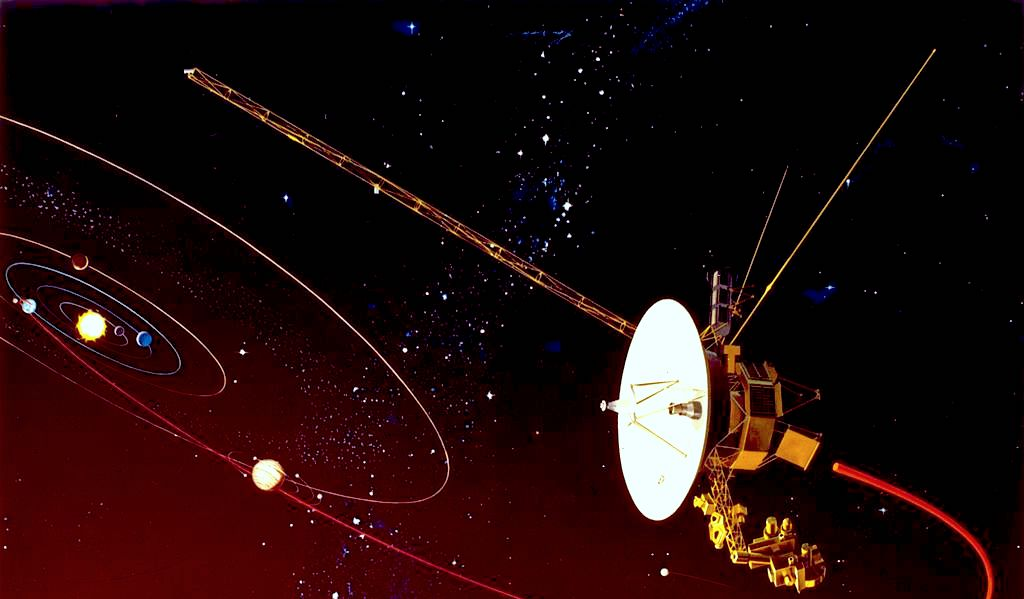
\includegraphics[height=1.6in]{images/voyager.jpg}
 \end{center}

    

     \end{frame}
  
  %%%%%%%%%%%%%%%%%%%%%%%%%%%%%%%%%%%%%%%%%%%%%%%%%%%%%%%%%%%%%%%%%%%



  %%%%%%%%%%%%%%%%%%%%%%%%%%%%%%%%%%%%%%%%%%%%%%%%%%%%%%%%%%%%%%%%%%%
  \begin{frame}
   % Insert frame title between curly braces
On the other hand\dots
 
 \pause
 \vspace{3mm}
 
 Knowing Dynamics can help us figure out accurate timing. Even if you plan to exaggerate your motion for 
 effect, it helps to start with reality and work from there.
  \end{frame}

%%%%%%%%%%%%%%%%%%%%%%%%%%%%%%%%%%%%%%%%%%%%%%%%%%%%%%%%%%%%%%%%%%%


  \subsection{Kinematics}


  \begin{frame}
    
  \textbf{Kinematics}
  
  \begin{columns}[c]
     \column{2.5in}  % slides are 3in high by 5in wide
    
     \begin{center}
      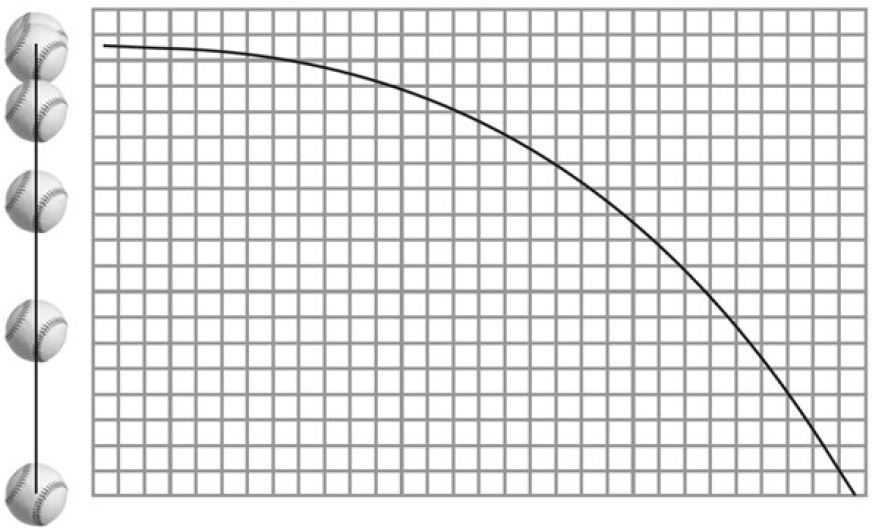
\includegraphics[height=1.6in]{images/motion_path.jpg}
    \end{center}
  
  
     \column{2in}
  


  \begin{itemize}
   \item Describes the motion path: Position vs. time $x(t), y(t)$ and $z(t)$ $\rightarrow$ timing and spacing. \pause
   
   \item There are three main quantities that describe the motion: \textcolor{mypink1}{acceleration}, \textcolor{mypink1}{velocity}
   and \textcolor{mypink1}{position}\pause
   
   \item The position is related with velocity and the velocity is related with acceleration. 
   \end{itemize}
  
   

  
     \end{columns}
  
  
  
   \end{frame}
  
  
  %%%%%%%%%%%%%%%%%%%%%%%%%%%%%%%%%%%%%%%%%%%%%%%%%%%%%%%%%%%%%%%%%%%
  

  \begin{frame}
   
You do this intuitively \dots \pause

\begin{center}
   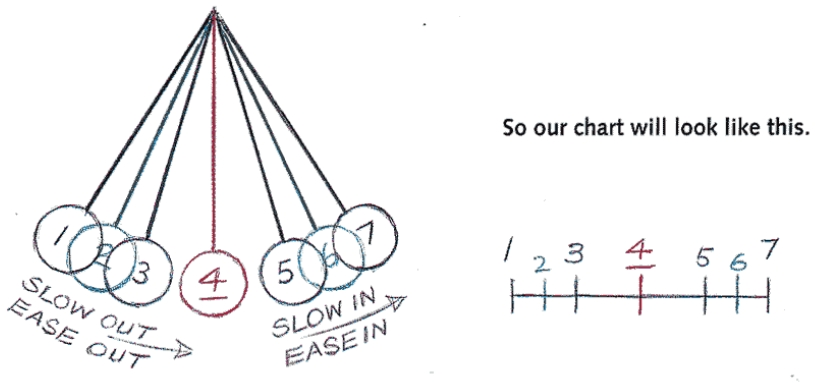
\includegraphics[height=1.6in]{images/space_timing.jpg}
 \end{center}
   

 \pause

 What is the right separation?
 \end{frame}

   %%%%%%%%%%%%%%%%%%%%%%%%%%%%%%%%%%%%%%%%%%%%%%%%%%%%%%%%%%%%%%%%%%%
  

   \begin{frame}
   
      You do this intuitively \dots \pause
      
      \begin{center}
         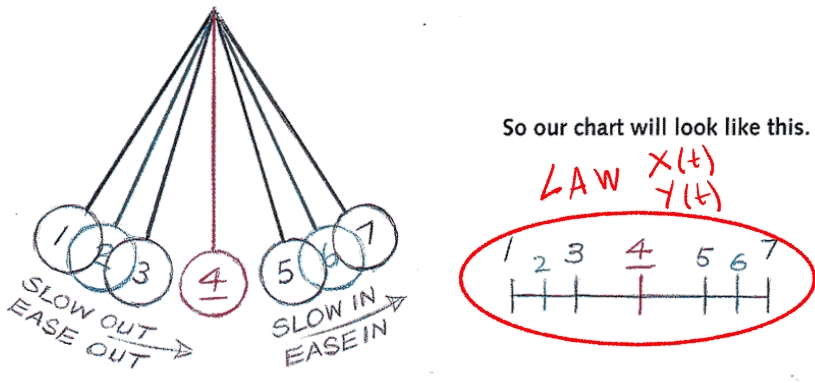
\includegraphics[height=1.6in]{images/space_timing2.jpg}
       \end{center}
         
      
       \pause
      
       What generate that exact separation? \pause \textcolor{mypink1}{FORCES \pause Dynamics}
       \end{frame}
       
 

       
 
   %%%%%%%%%%%%%%%%%%%%%%%%%%%%%%%%%%%%%%%%%%%%%%%%%%%%%%%%%%%%%%%%%%%

  \begin{frame}
   We are going to find those laws, but first, we need to review some Math basics: 
  
  \pause
  \vspace{3mm}
  
  \begin{itemize}
  \item Frames of Reference 
  \item escalar and vectors
  \item funcions
  \item trigonometry
  \end{itemize}
  
  
  
  
  
   \end{frame}

  %%%%%%%%%%%%%%%%%%%%%%%%%%%%%%%%%%%%%%%%%%%%%%%%%%%%%%%%%%%%%%%%%%%




   \begin{frame}

    \textbf{Frame of reference}
    \vspace{3mm}
    
     When we want to describe the motion of a body, the first thing we need to define 
    is a coordinate system.
     
    
    
    
    
       \begin{columns}[c]
       \column{2in}  % slides are 3in high by 5in wide
      
    \pause
    \begin{itemize}
    \item The position is determined by the numbers $(x,y,z)$ 
    \pause
    \item Defining these 3 numbers plus a time scale we can represent  the position vs time. 
    \end{itemize}
    
       \column{2.5in}
      \begin{center}
      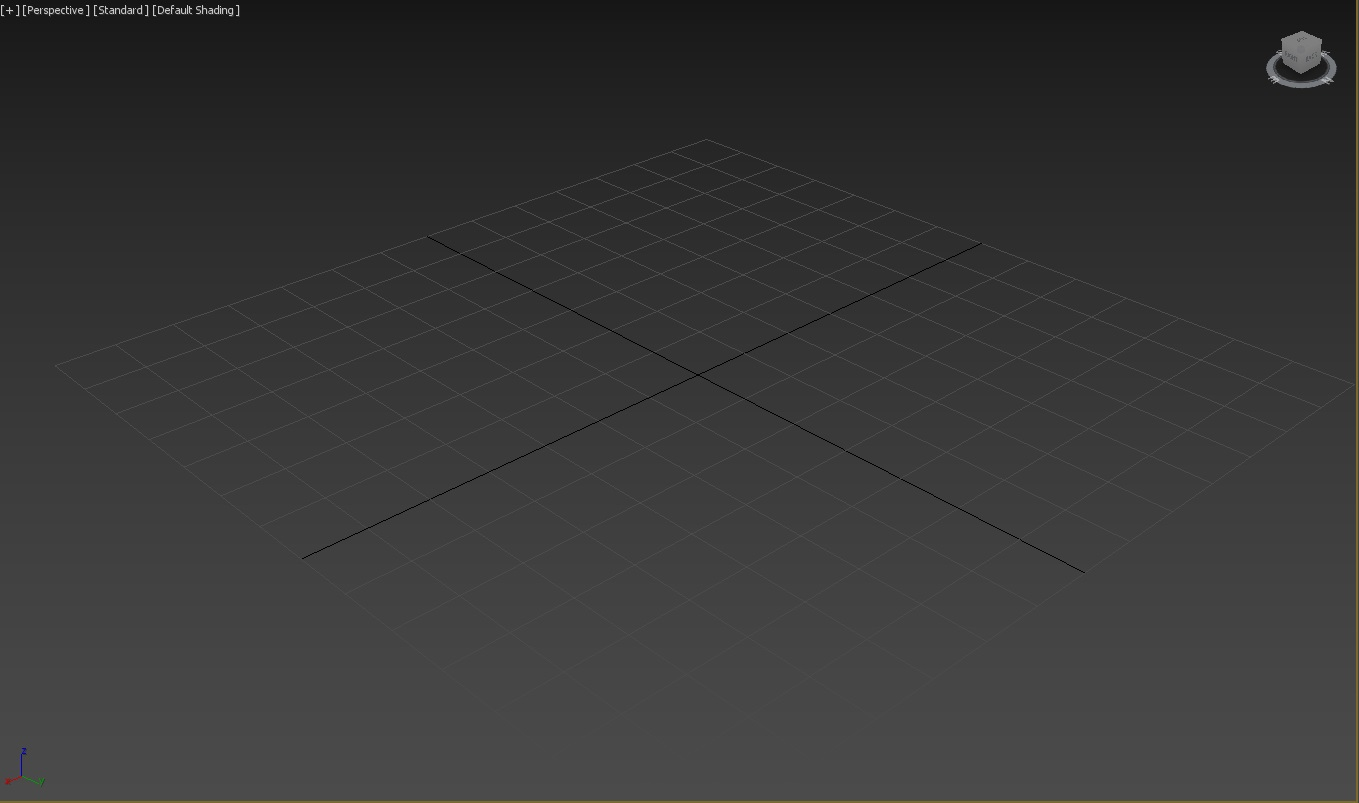
\includegraphics[height=1.6in]{images/reference_frame.jpg}
    \end{center}
    
       \end{columns}
    \pause
    
      \begin{center}
      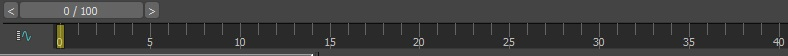
\includegraphics[height=0.3in]{images/time_line.jpg}
    \end{center}
    
     \end{frame}
    
    
    
    %%%%%%%%%%%%%%%%%%%%%%%%%%%%%%%%%%%%%%%%%%%%%%%%%%%%%%%%%%%%%%%%%%%
  
   \begin{frame}
   
      Another example of a reference system \dots
 
      \begin{center}
       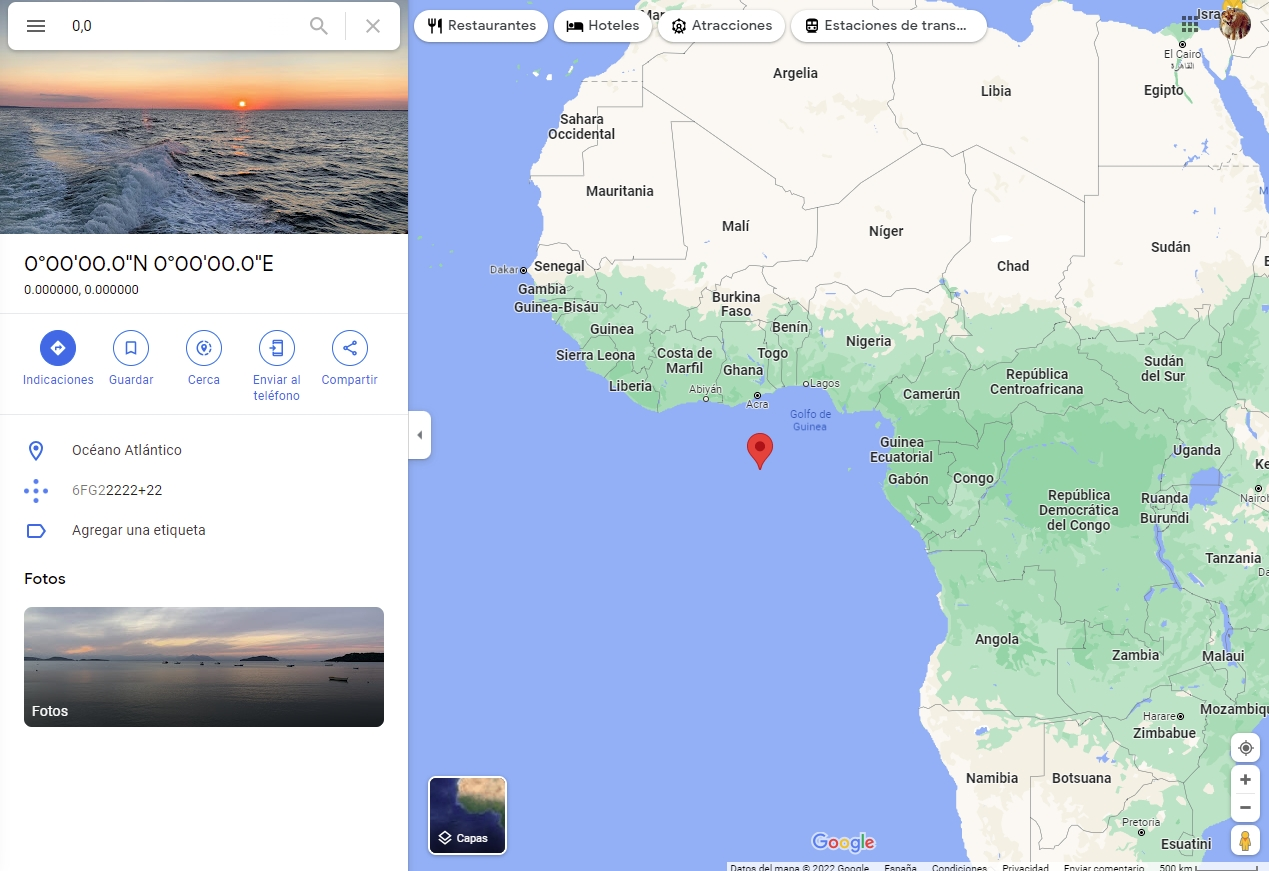
\includegraphics[height=1.9in]{images/reference_map.jpg}
     \end{center}
 

      \end{frame}
  %%%%%%%%%%%%%%%%%%%%%%%%%%%%%%%%%%%%%%%%%%%%%%%%%%%%%%%%%%%%%%%%%%%  
    

    
    
  \begin{frame}
   Vectors
   
         % Insert frame title between curly braces
   \begin{itemize}
   \item Some physical quantities, such as time, temperature, mass, and density, can be
   described completely by a single number with a unit.
   \pause
   \item But many other important quantities in physics have a direction associated with them and cannot be
   described by a single number %(displacement, velocity, acceleration, force, ...)
   \end{itemize}
   
   
   
    \end{frame}
    %%%%%%%%%%%%%%%%%%%%%%%%%%%%%%%%%%%%%%%%%%%%%%%%%%%%%%%%%%%%%%%%%%%

    
    
  \begin{frame}
For example, you use vectors to determine the direction of a curve in vectorial illustration\dots \pause

\begin{center}
   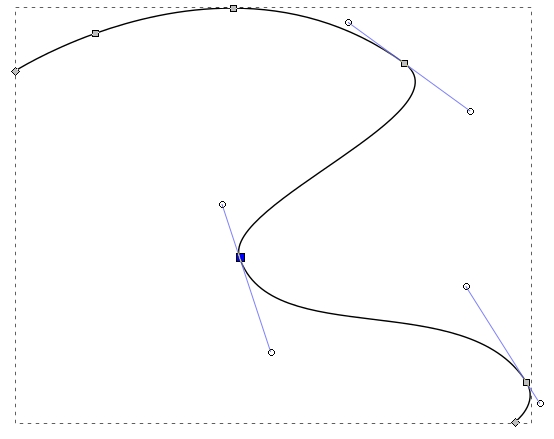
\includegraphics[height=1.9in]{images/vectorial_illustration.jpg}
 \end{center}
   
   
    \end{frame}

%%%%%%%%%%%%%%%%%%%%%%%%%%%%%%%%%%%%%%%%%%%%%%%%%%%%%%%%%%%%%%%%%%%
\begin{frame}
   Another examples of vectors? \pause

   \begin{itemize}
      \item velocity
      \item acceleration
      \item force 
      \item \dots
   \end{itemize}

   \pause

How do we use them?
      
\end{frame}


%%%%%%%%%%%%%%%%%%%%%%%%%%%%%%%%%%%%%%%%%%%%%%%%%%%%%%%%%%%%%%%%%%%

     \begin{frame}
      Vectors
      
            % Insert frame title between curly braces
      \begin{itemize}
      \item When a physical quantity is described by a single number, we call it a \textbf{scalar
      quantity}.
      \pause
      \item A \textbf{vector quantity} has both a magnitude and a direction in space.
      \pause 
      \item We represent a vector quantity  by a single letter, italic type with an arrow above it:  $\vec{v}$
      \end{itemize}
      
      
      
       \end{frame}
      %%%%%%%%%%%%%%%%%%%%%%%%%%%%%%%%%%%%%%%%%%%%%%%%%%%%%%%%%%%%%%%%%%%
      
      \begin{frame}
      
      
      
         \begin{columns}[c]
         \column{2.5in}  % slides are 3in high by 5in wide
        
      
      \begin{itemize}
      \item Vectors are represented by arrows in diagrams. 
      
      \item the magnitude is just the length of the arrow.
      
      
      \item $\vec{A}=\vec{A}'$
      \end{itemize}
      
      
         \column{2in}
      
      
        \begin{center}
        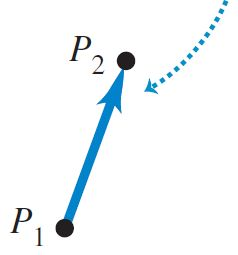
\includegraphics[height=1.5in]{images/vector.jpg}
      \end{center}
      
      
         \end{columns}
      
      
      
      
      \end{frame}
      
      
      %%%%%%%%%%%%%%%%%%%%%%%%%%%%%%%%%%%%%%%%%%%%%%%%%%%%%%%%%%%%%%%%%%%


      \begin{frame}



        \begin{columns}[c]
        \column{2.5in}  % slides are 3in high by 5in wide
       
     
     \begin{itemize}
     
     
     \item If two vectors have the same magnitude and the same direction, they are equal, 
     no matter where they are located in space.
     
     \item $\vec{A}=\vec{A}'$
     \end{itemize}
     
     
        \column{2in}
     
     
       \begin{center}
       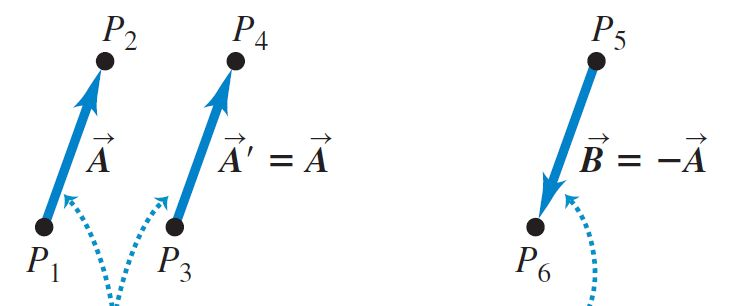
\includegraphics[height=1.5in]{images/paralel_vec.jpg}
     \end{center}
     
     
        \end{columns}
     
     
     
     
     \end{frame}




     \begin{frame}




      \begin{columns}[c]
      \column{2in}  % slides are 3in high by 5in wide
     
   \begin{itemize}
   \item We define the negative of a vector as a vector having the
   same magnitude as the original vector but the opposite direction.
   
   \item $\vec{A}=-\vec{B}$
   
   \item When two vectors are parallel and have opposite directions,
   we say that they are antiparallel.
   \end{itemize}
   
   
      \column{2in}
   
   
   
     \begin{center}
     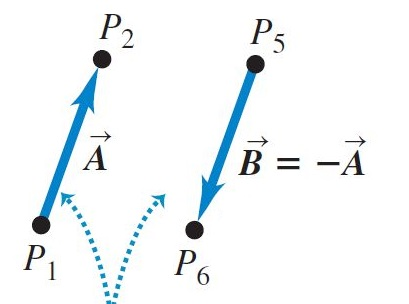
\includegraphics[height=1.7in]{images/antiparalel_vec.jpg}
   \end{center}
   
   
      \end{columns}
   
   
   
   
   \end{frame}


   %%%%%%%%%%%%%%%%%%%%%%%%%%%%%%%%%%%%%%%%%%%%%%%%%%%%%%%%%%%%%%%%%%%

\begin{frame}

  We usually represent the magnitude of a vector  by the same letter used for the vector
  and vertical bars on both sides:
  \pause
  
  \begin{equation}
  (magnitude~of~\vec{A}=\lvert \vec{A} \rvert)
  \end{equation}
  
  \pause 
  \begin{itemize}
  \item The magnitude of a vector is a positive scalar (a positive number). 
  \pause
  \item A vector can never be equal to a scalar because they are different kind of quantities.
  \end{itemize}
  
  \end{frame}
  
  
  
  %%%%%%%%%%%%%%%%%%%%%%%%%%%%%%%%%%%%%%%%%%%%%%%%%%%%%%%%%%%%%%%%%%%

  \begin{frame}
    Displacement 
    \vspace{3 mm}
    
    
    
       \begin{columns}[c]
       \column{2in}  % slides are 3in high by 5in wide
      
    
    
    \begin{itemize}
    \item Displacement is simply a change in the position of an object. 
    
    
    \end{itemize}
    
    
       \column{2in}
    
    
    
    
      \begin{center}
      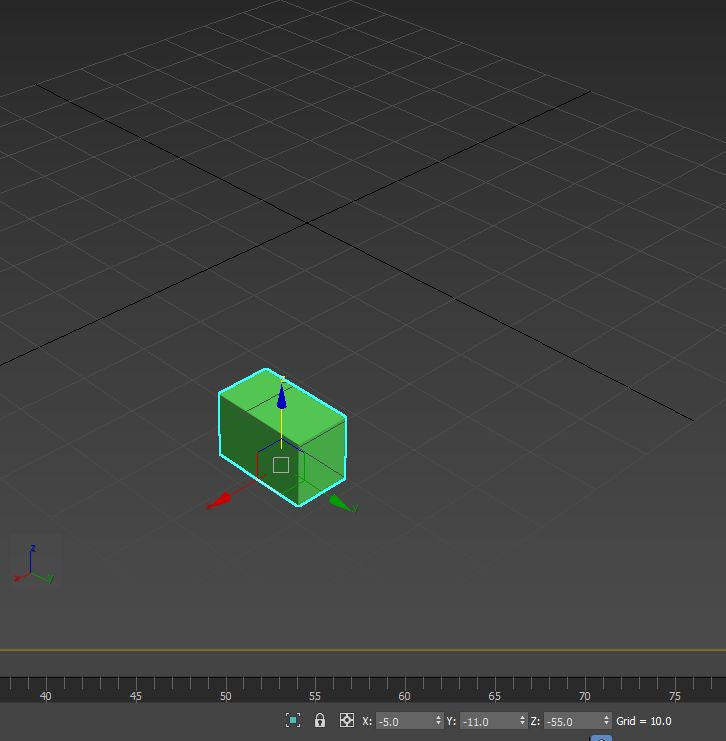
\includegraphics[height=1.7in]{images/dis3d1.jpg}
    \end{center}
    
    
       \end{columns}
    
     \end{frame}
    %%%%%%%%%%%%%%%%%%%%%%%%%%%%%%%%%%%%%%%%%%%%%%%%%%%%%%%%%%%%%%%%%%%


    \begin{frame}
      Displacement 
      \vspace{3 mm}
      
      
      
         \begin{columns}[c]
         \column{2in}  % slides are 3in high by 5in wide
        
      
      
      \begin{itemize}
      \item Displacement is simply a change in the position of an object. 
      
      
      \end{itemize}
      
      
         \column{2in}
      
      
      
      
        \begin{center}
        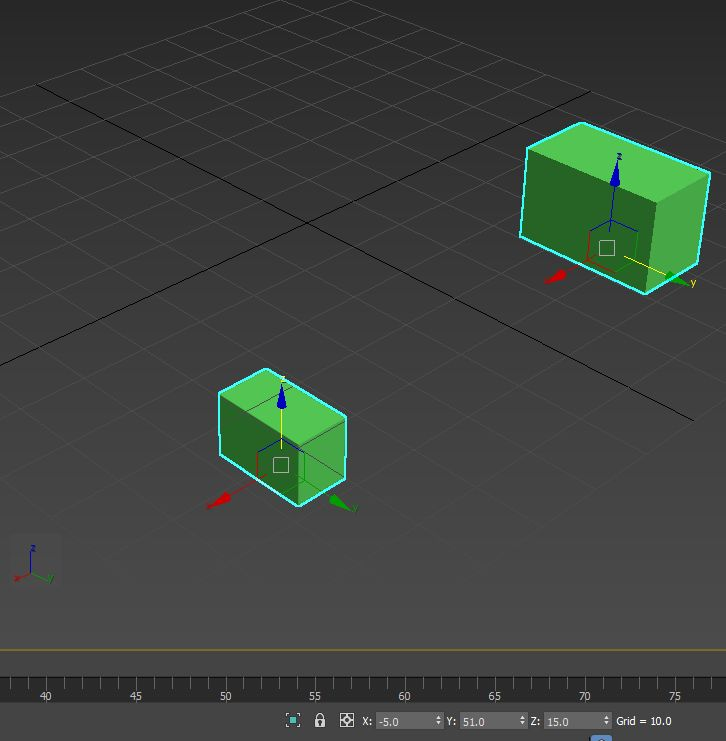
\includegraphics[height=1.7in]{images/dis3d2.jpg}
      \end{center}
      
      
         \end{columns}
      
       \end{frame}
      %%%%%%%%%%%%%%%%%%%%%%%%%%%%%%%%%%%%%%%%%%%%%%%%%%%%%%%%%%%%%%%%%%%



      \begin{frame}
        Displacement 
        \vspace{3 mm}
        
        
        
           \begin{columns}[c]
           \column{2in}  % slides are 3in high by 5in wide
          
        
        
        \begin{itemize}
        \item Displacement is simply a change in the position of an object. 
        
        \item It  is a vector because we must state how far the object moves and the direction.
        
        
        
        \end{itemize}
        
        
           \column{2in}
        
        
        
        
          \begin{center}
          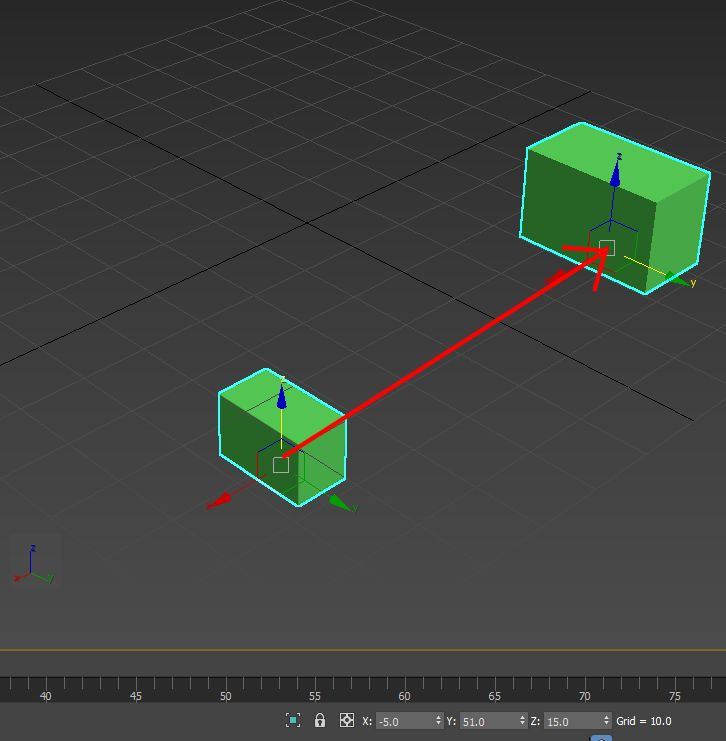
\includegraphics[height=1.7in]{images/dis3d3.jpg}
        \end{center}
        
        
           \end{columns}
        
         \end{frame}
        
        %%%%%%%%%%%%%%%%%%%%%%%%%%%%%%%%%%%%%%%%%%%%%%%%%%%%%%%%%%%%%%%%%%%

        
\begin{frame}
  Displacement 
  \vspace{3 mm}
  
  
  
     \begin{columns}[c]
     \column{2in}  % slides are 3in high by 5in wide
    
  
  
  \begin{itemize}
  \item Displacement is simply a change in the position of an object. 
  
  \item It  is a vector because we must state how far the object moves and the direction.
  
  \item The displacement only depend on the initial and final positions.
  \end{itemize}
  
  
     \column{2in}
  
  
  
  
    \begin{center}
    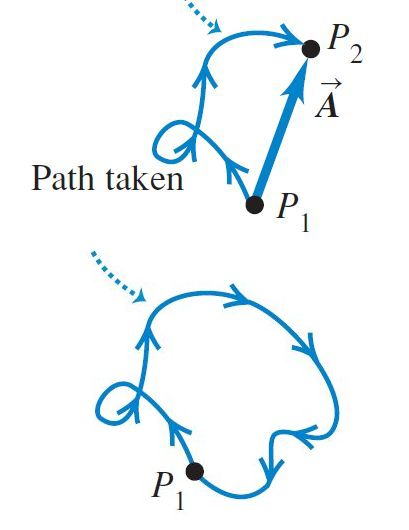
\includegraphics[height=2.in]{images/dis2.jpg}
  \end{center}
  
  
     \end{columns}
  
   \end{frame}
  %%%%%%%%%%%%%%%%%%%%%%%%%%%%%%%%%%%%%%%%%%%%%%%%%%%%%%%%%%%%%%%%%%%




  \begin{frame}

    Operations with vector: Addition and subtraction 
    
    \vspace{3 mm}
    \pause
    
    
       \begin{columns}[c]
       \column{2in}  % slides are 3in high by 5in wide
    
    
    Suppose a particle undergoes a displacement $\vec{A}$ followed by a second displacement$\vec{B}$. 
    The final result is the same as if the particle had started at the same initial
    point and undergone a single displacement $\vec{C}$.
    
    
      
       \column{2in}
    
    
    
    
      \begin{center}
      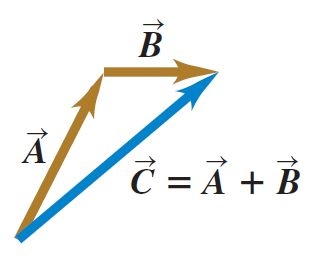
\includegraphics[height=1.7in]{images/vectorsum1.jpg}
    \end{center}
    
    
       \end{columns}
    
    
    \end{frame}
    
    %%%%%%%%%%%%%%%%%%%%%%%%%%%%%%%%%%%%%%%%%%%%%%%%%%%%%%%%%%%%%%%%%%%



    \begin{frame}

      Operations with vector: Addition and subtraction
      
      \vspace{3 mm}
      
      
      
         \begin{columns}[c]
         \column{2in}  % slides are 3in high by 5in wide
      
      
      \begin{equation*}
      \vec{C}=\vec{A}+\vec{B}
      \end{equation*}
      
      \begin{itemize}
      \item vector addition obeys the commutative law
      
      \item $\vec{A}+\vec{B}=\vec{B}+\vec{A}$
      
      \item  note that the magnitude of $\lvert C \rvert \leq\lvert A \rvert+\lvert B \rvert$
      \end{itemize}
      
        
         \column{2in}
      
      
      
      
        \begin{center}
        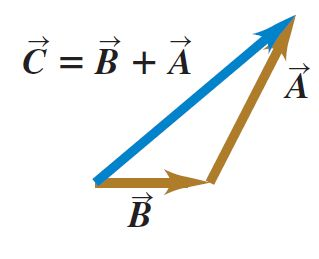
\includegraphics[height=1.7in]{images/vectorsum2.jpg}
      \end{center}
      
      
         \end{columns}
      
      
      \end{frame}



%%%%%%%%%%%%%%%%%%%%%%%%%%%%%%%%%%%%%%%%%%%%%%%%%%%%%%%%%%%%%%%%%%%


\begin{frame}

  Sum of more than two vector:
  
  
  
  
     \begin{columns}[c]
     \column{2in}  % slides are 3in high by 5in wide
    
  
  \begin{equation*}
  \vec{R}=(\vec{A}+\vec{B})+\vec{C}=\vec{D}+\vec{C}
  \end{equation*}
  or
  
  \begin{equation*}
  \vec{R}=\vec{A}+(\vec{B}+\vec{C})=\vec{A}+\vec{E}
  \end{equation*}
  
  
  
     \column{2in}
  
  
  
  
    \begin{center}
    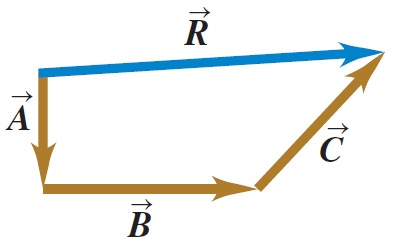
\includegraphics[height=1.5in]{images/sum_of_more_vec.jpg}
  \end{center}
  
  
     \end{columns}
  
  
  
  \end{frame}


%%%%%%%%%%%%%%%%%%%%%%%%%%%%%%%%%%%%%%%%%%%%%%%%%%%%%%%%%%%%%%%%%%%


\begin{frame}

  We define the difference of two vectors $\vec{A}$ and $\vec{B}$ to be the vector sum of $\vec{A}$ and $-\vec{B}$:
 
 
 \begin{equation*}
 \vec{A}-\vec{B}=\vec{A}+(-\vec{B})
 \end{equation*}
 
 \vspace{5mm}
 
  \begin{center}
   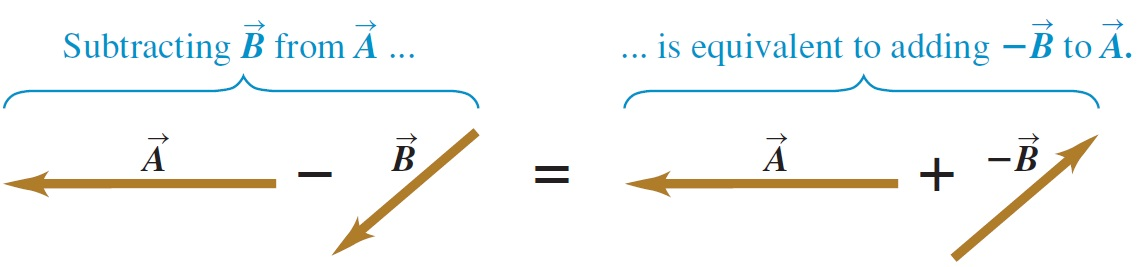
\includegraphics[height=0.9in]{images/subs_vecs.jpg}
 \end{center}
 
 
 
 \end{frame}
 
%%%%%%%%%%%%%%%%%%%%%%%%%%%%%%%%%%%%%%%%%%%%%%%%%%%%%%%%%%%%%%%%%%%


\begin{frame}

  A vector can be multiplied by a positive (negative) scalar quantity. The result is a vector 
  in the same direction (opposite) as the vector but with a different magnitud.
  
  The magnitude is $\lvert c \rvert \lvert \vec{A} \rvert$
  \end{frame}
  
  %%%%%%%%%%%%%%%%%%%%%%%%%%%%%%%%%%%%%%%%%%%%%%%%%%%%%%%%%%%%%%%%%%%
  
  \begin{frame}
  
  EXAMPLE 1: Adding two vectors that are perpendicular
  \vspace{3 mm}
  
  A cross-country skier skis $1.00~km$ north and then $2.00~km$ east on
  a horizontal snowfield. How far and in what direction is she from
  the starting point?
  
  
  
  
  
  \end{frame}





%%%%%%%%%%%%%%%%%%%%%%%%%%%%%%%%%%%%%%%%%%%%%%%%%%%%%%%%%%%%%%%%%%%

\begin{frame}



  \begin{columns}[c]
   \column{2in}  % slides are 3in high by 5in wide

   \begin{center}
      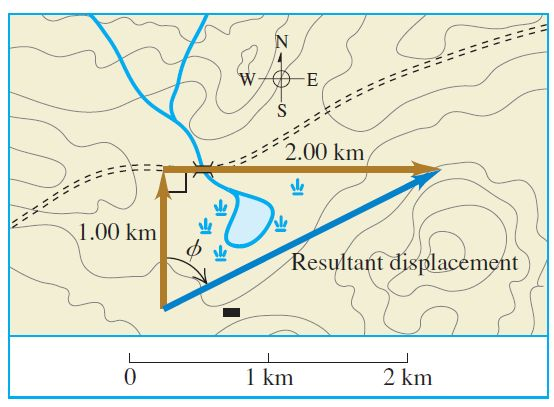
\includegraphics[height=1.7in]{images/perp_vec.jpg}
    \end{center}
    


  
   \column{2.7in}

 

Distance from the starting point:
\pause

\begin{equation*}
\sqrt{(1.00~km)^2+(2.00~km)^2}=2.24~km
\end{equation*}

\vspace{3 mm}

\pause

direction:

\pause

\begin{equation*}
tan \phi =\frac{opposite~side}{Adjacent~side}=\frac{2.00~km}{1.00~km}
\end{equation*}
\pause


\begin{equation*}
 \phi =63.4^{\circ}
\end{equation*}


   \end{columns}





\end{frame}

%%%%%%%%%%%%%%%%%%%%%%%%%%%%%%%%%%%%%%%%%%%%%%%%%%%%%%%%%%%%%%%%%%%


\begin{frame}
EXAMPLE 2: Test Your Understanding 
\vspace{3 mm}

Two displacement vectors, $\vec{u}$ and $\vec{v}$ have magnitudes 3 and 4. Which of the following could
be the magnitude of the difference vector (There may be more than one correct answer.)
\vspace{3 mm}

\begin{itemize}
\item  9 m
\item 7 m
\item  5 m
\item 1 m
\item 0 m
\item -1 m
 \end{itemize}
\end{frame}

\subsection{Doing vector calculation using components }

  
\begin{frame}
\begin{itemize}
\item Calculations with right triangles work only when the two vectors are perpendicular.
\pause
\item Measuring a diagram offers only very limited accuracy.
\pause
\item So we need a simple but general method for adding vectors.
\pause
\item  This is called the
method of components.
\end{itemize}

\end{frame}

%%%%%%%%%%%%%%%%%%%%%%%%%%%%%%%%%%%%%%%%%%%%%%%%%%%%%%%%%%%%%%%%%%%


\begin{frame}

COMPONENTS OF VECTORS



\begin{columns}
\column{0.5\textwidth}

\begin{itemize}
\item Consider a rectangular (Cartesian) coordinate system of axes \pause

\item We then draw the vector with its tail at O \pause

\item We can represent any vector in the xy-plane as the sum of a vector in the x-axis and a vector 
in the y-axis \pause
\end{itemize}

\begin{equation}
\vec{A}=\vec{A}_x+\vec{A}_y
\end{equation}
\pause

\column{0.5\textwidth}

\begin{center}
     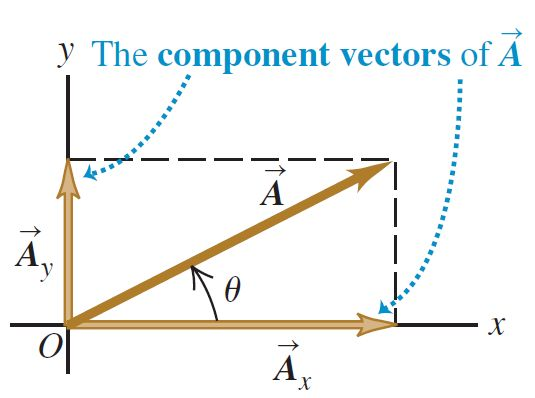
\includegraphics[width=1.\textwidth]{images/component_vec.jpg}      
     \end{center}


\end{columns}



\end{frame}

%%%%%%%%%%%%%%%%%%%%%%%%%%%%%%%%%%%%%%%%%%%%%%%%%%%%%%%%%%%%%%%%%%%


\begin{frame}



\begin{itemize}
\item Since each component vector lies along a coordinate-axis direction, we need
only a single number to describe each one.

\pause

\item When $\vec{A}_x$ points in the positive x-direction, we define the number $A_x$,  $A_x=\lvert \vec{A}_x \rvert$

\pause


\item  When $\vec{A}_x$ points in the negative x-direction, we define the number $A_x$,  $A_x=-\lvert \vec{A}_x \rvert$

\pause


\item We define the number $\vec{A}_y$ in the same way
\end{itemize}

\vspace{5 mm}
\pause

 The two numbers $A_x$ and $A_y$ are called the components of $\vec{A}$.
\pause

\vspace{5 mm}
We represent $\vec{A}$ using its components as:
\begin{equation}
\vec{A}=(A_x,A_y)
\end{equation}

 \end{frame}
 
 %%%%%%%%%%%%%%%%%%%%%%%%%%%%%%%%%%%%%%%%%%%%%%%%%%%%%%%%%%%%%%%%%%%


\begin{frame}



\begin{itemize}
\item If we know the direction and the magnitude of a vector, we can know the components.
\end{itemize}





\begin{columns}
\column{0.5\textwidth}





\begin{equation*}
 \frac{A_x}{A}=cos \theta, ~and~  \frac{A_y}{A}=sin \theta 
\end{equation*}



\begin{equation*}
 A_x=A cos \theta,~  and~  A_y=A sin \theta 
\end{equation*}

\begin{equation*}
\rightarrow \vec{A}=\vec{A}_x+\vec{A}_y
\end{equation*}


\column{0.5\textwidth}

\begin{center}
     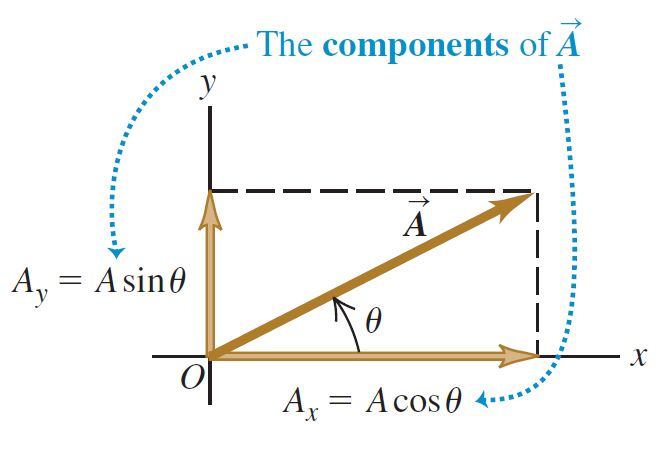
\includegraphics[width=1.\textwidth]{images/component_vec2.jpg}      
     \end{center}


\end{columns}




 \end{frame}

%%%%%%%%%%%%%%%%%%%%%%%%%%%%%%%%%%%%%%%%%%%%%%%%%%%%%%%%%%%%%%%%%%%
\begin{frame}



\vspace{5mm}

Finding a vector’s magnitude and direction from its components.
\vspace{5mm}

\begin{equation}
A=\sqrt{A^2_x+A^2_y}
\end{equation}

\begin{equation}
tan \theta =\frac{A_y}{A_x} \ \ and \ \ \theta =arctan (\frac{A_y}{A_x})
\end{equation}

 \end{frame}


%%%%%%%%%%%%%%%%%%%%%%%%%%%%%%%%%%%%%%%%%%%%%%%%%%%%%%%%%%%%%%%%%%%

\begin{frame}




Multiplying a vector by a scalar.

\begin{equation}
\vec{D}=c\vec{A}
\end{equation}

\begin{equation}
D_x =c{A_x} \ \ and \ \ D_y =c{A_y}
\end{equation}


 \end{frame}
%%%%%%%%%%%%%%%%%%%%%%%%%%%%%%%%%%%%%%%%%%%%%%%%%%%%%%%%%%%%%%%%%%%

\begin{frame}




 Using the components to calculate the vector sum







\begin{columns}
\column{0.5\textwidth}


\begin{equation*}
\vec{R}=\vec{A}+\vec{B}
\end{equation*}

\begin{equation*}
R_x =A_x+B_x
\end{equation*}

\begin{equation*}
R_y =A_y+B_y
\end{equation*}



\column{0.5\textwidth}

\begin{center}
     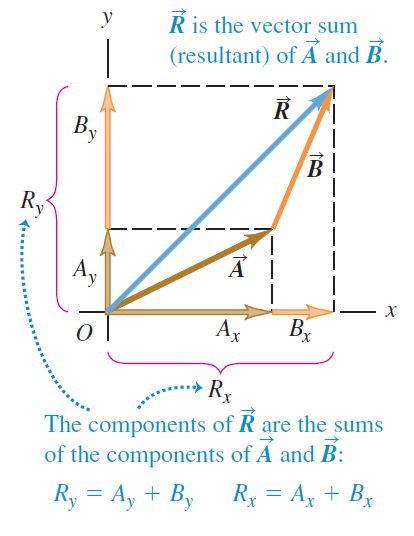
\includegraphics[width=1.\textwidth]{images/vector_sum.jpg}      
     \end{center}


\end{columns}




 \end{frame}




%%%%%%%%%%%%%%%%%%%%%%%%%%%%%%%%%%%%%%%%%%%%%%%%%%%%%%%%%%%%%%%%%%%




\begin{frame}


  EXAMPLE:
  
  
  
  
  
  
  
  \begin{columns}
  \column{0.5\textwidth}
  
  You are using vector sums to move objects in 3ds Max all the time...
  
  
  \column{0.5\textwidth}
  
  \begin{center}
       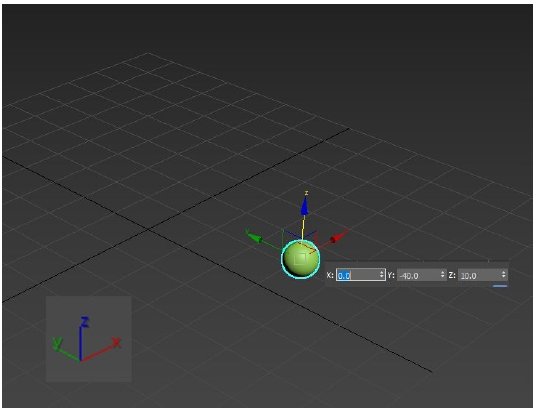
\includegraphics[width=1.1\textwidth]{images/exampleVS1.jpg}      
       \end{center}
  
  
  \end{columns}
  
  
  
  
   \end{frame}
  
%%%%%%%%%%%%%%%%%%%%%%%%%%%%%%%%%%%%%%%%%%%%%%%%%%%%%%%%%%%%%%%%%%%

\begin{frame}


  EXAMPLE:
  
  
  
  
  
  
  
  \begin{columns}
  \column{0.5\textwidth}
  
  Position vector
  
  
  \column{0.5\textwidth}
  
  \begin{center}
       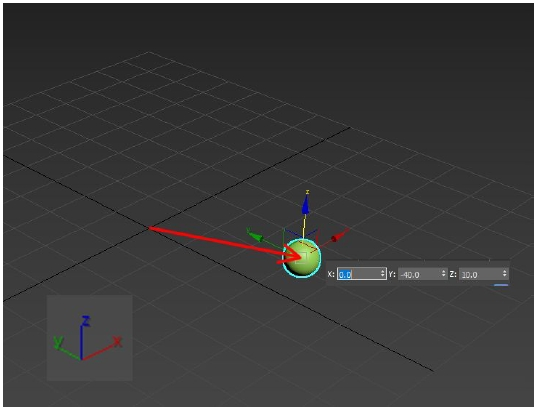
\includegraphics[width=1.1\textwidth]{images/exampleVS2.jpg}      
       \end{center}
  
  
  \end{columns}
  
  
  
  
   \end{frame}
  
  
  %%%%%%%%%%%%%%%%%%%%%%%%%%%%%%%%%%%%%%%%%%%%%%%%%%%%%%%%%%%%%%%%%%%
  
  \begin{frame}
  
  
  EXAMPLE:
  
  
  
  
  
  
  
  \begin{columns}
  \column{0.5\textwidth}
  
  Displacement Vector
  
  
  \column{0.5\textwidth}
  
  \begin{center}
       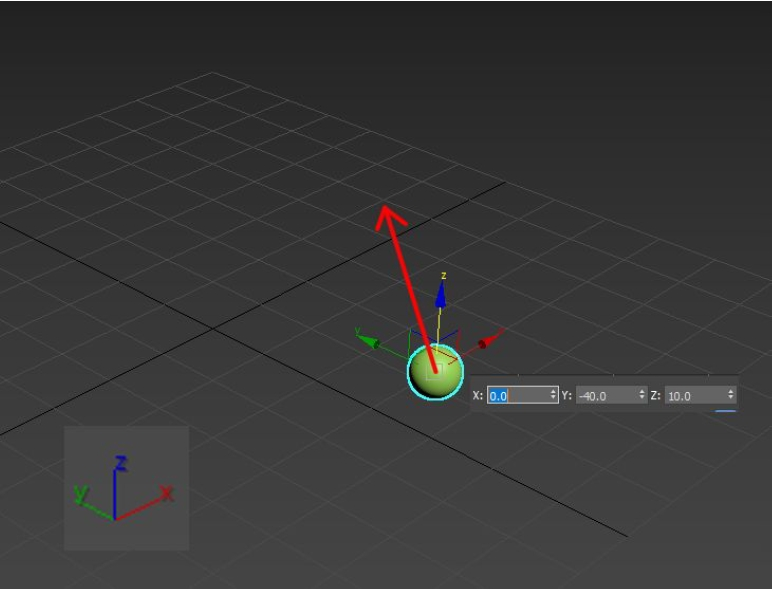
\includegraphics[width=1.1\textwidth]{images/exampleVS3.jpg}      
       \end{center}
  
  
  \end{columns}
  
  
  
  
   \end{frame}
  
  %%%%%%%%%%%%%%%%%%%%%%%%%%%%%%%%%%%%%%%%%%%%%%%%%%%%%%%%%%%%%%%%%%%
  
  \begin{frame}
  
  
  EXAMPLE:
  
  
  
  
  
  
  
  \begin{columns}
  \column{0.5\textwidth}
  
   Displacement Vector
  
  
  \column{0.5\textwidth}
  
  \begin{center}
       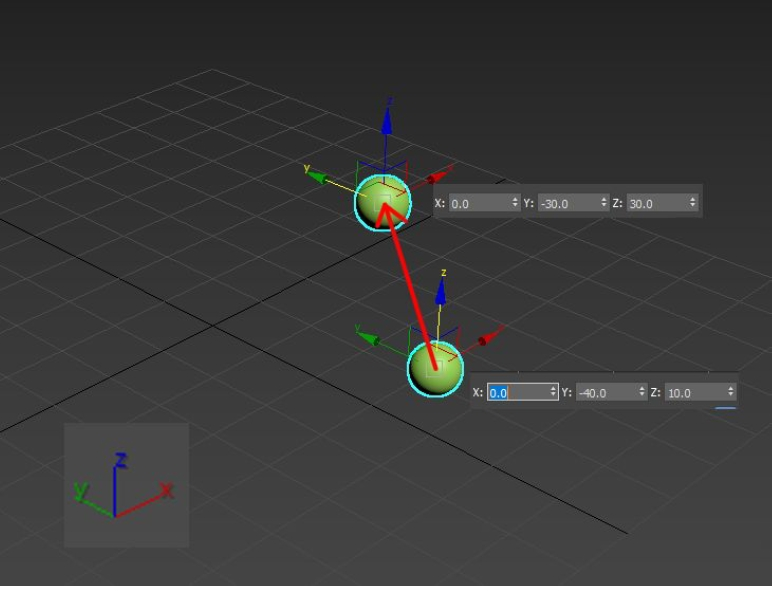
\includegraphics[width=1.1\textwidth]{images/exampleVS4.jpg}      
       \end{center}
  
  
  \end{columns}
  
  
  
  
   \end{frame}
  
  %%%%%%%%%%%%%%%%%%%%%%%%%%%%%%%%%%%%%%%%%%%%%%%%%%%%%%%%%%%%%%%%%%%
  
  \begin{frame}
  
  
  EXAMPLE:
  
  
  
  
  
  
  
  \begin{columns}
  \column{0.5\textwidth}
  
  Final Position=Position Vector + Displacement Vector
  
  
  \column{0.5\textwidth}
  
  \begin{center}
       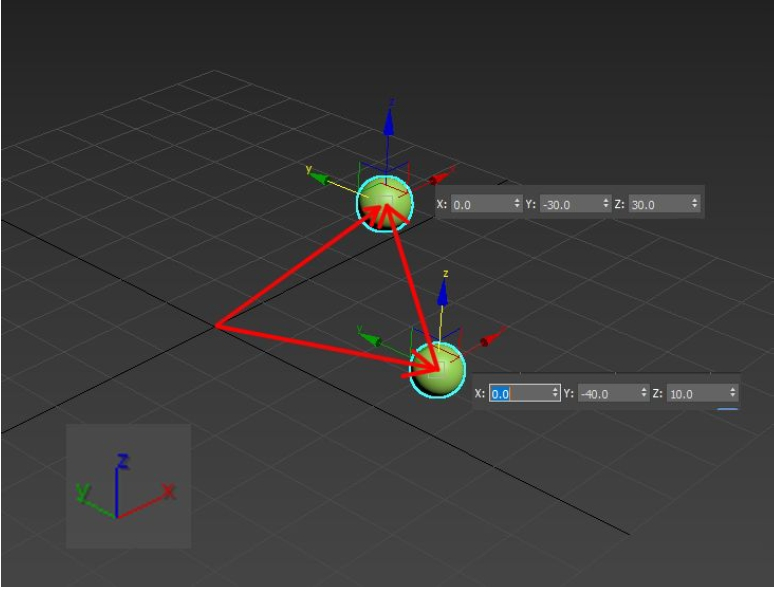
\includegraphics[width=1.1\textwidth]{images/exampleVS5.jpg}      
       \end{center}
  
  
  \end{columns}
  
  
  
  
   \end{frame}
  
  %%%%%%%%%%%%%%%%%%%%%%%%%%%%%%%%%%%%%%%%%%%%%%%%%%%%%%%%%%%%%%%%%%%
  
  \begin{frame}
  
  
  EXAMPLE:
  
  
  
  
  
  
  
  \begin{columns}
  \column{0.5\textwidth}
  
  A more elegant notation...
  
  \begin{equation}
  \vec{r}_f=\vec{r}_i+\Delta \vec{ r}
  \end{equation}
  
  
  \column{0.5\textwidth}
  
  \begin{center}
       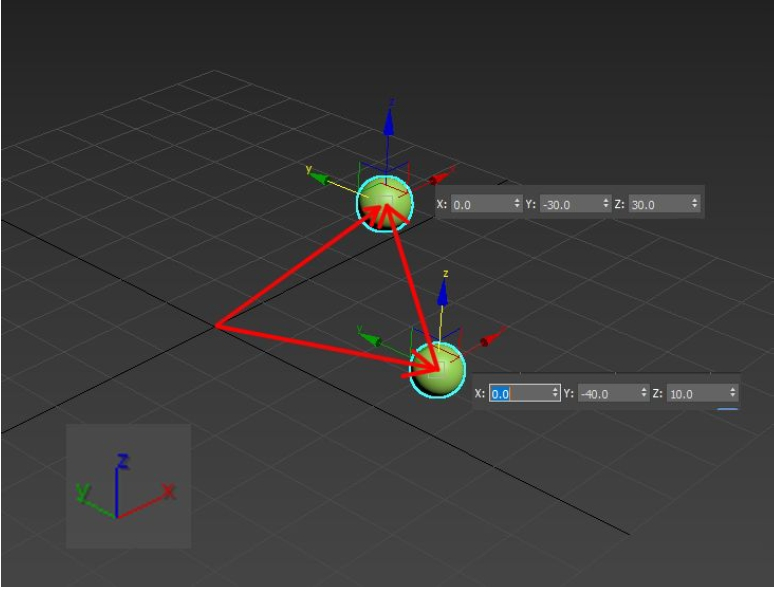
\includegraphics[width=1.1\textwidth]{images/exampleVS5.jpg}      
       \end{center}
  
  
  \end{columns}
  
  
  
  
   \end{frame}
  
  %%%%%%%%%%%%%%%%%%%%%%%%%%%%%%%%%%%%%%%%%%%%%%%%%%%%%%%%%%%%%%%%%%%
  
  \begin{frame}
  
  
  EXAMPLE:
  
  
  
  
  
  
  
  \begin{columns}
  \column{0.5\textwidth}
  
  so, the displacement vector is...
  
  \begin{equation}
  \Delta \vec{ r}+=\vec{r}_f-\vec{r}_i
  \end{equation}
  
  
  \column{0.5\textwidth}
  
  \begin{center}
       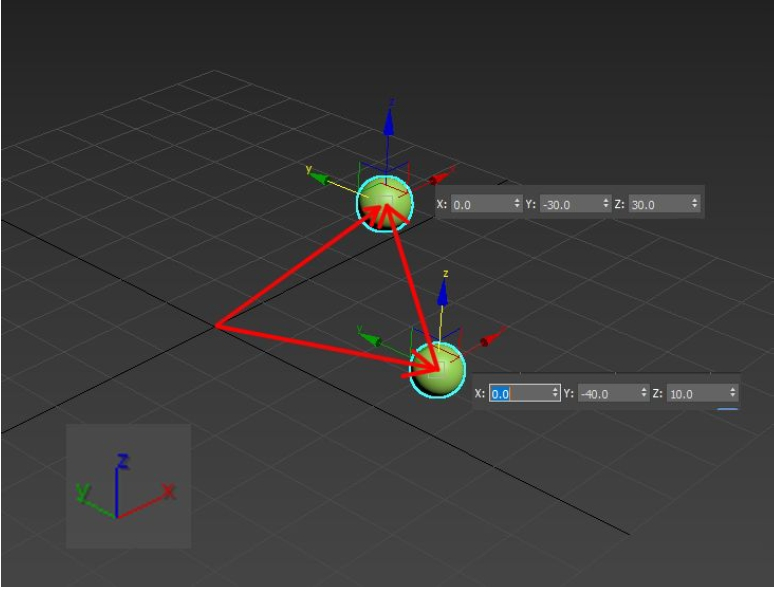
\includegraphics[width=1.1\textwidth]{images/exampleVS5.jpg}      
       \end{center}
  
  
  \end{columns}
  
  
  
  
   \end{frame}
  
  
  %%%%%%%%%%%%%%%%%%%%%%%%%%%%%%%%%%%%%%%%%%%%%%%%%%%%%%%%%%%%%%%%%%%



\begin{frame}


In general, we use the symbol $\Delta$ to represent the change of a magnitude...




 \end{frame}




%%%%%%%%%%%%%%%%%%%%%%%%%%%%%%%%%%%%%%%%%%%%%%%%%%%%%%%%%%%%%%%%%%%

\begin{frame}



   \begin{columns}[c]
   \column{2in}  % slides are 3in high by 5in wide

\begin{itemize}
\item In the previous definitions we measure the angles as in the figure.
\end{itemize}


  
   \column{2in}




  \begin{center}
  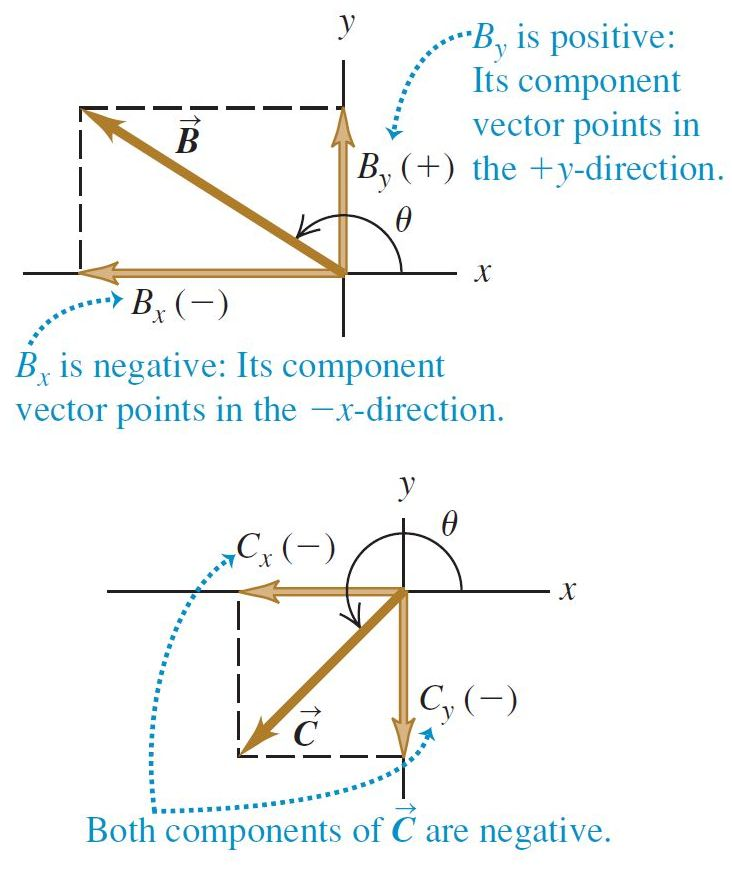
\includegraphics[height=2.5in]{images/component_vec3.jpg}
\end{center}


   \end{columns}


 \end{frame}



%%%%%%%%%%%%%%%%%%%%%%%%%%%%%%%%%%%%%%%%%%%%%%%%%%%%%%%%%%%%%%%%%%%

\begin{frame}


EXAMPLE:  (a) What are the x and y components of vector in the figure?
The magnitude of the vector $\vec{D}$  is $D=3.00~m$, and the angle $\alpha=45^\circ$. 
(b) What are the x- and y-components of vector $\vec{E}$  in? The magnitude of the vector is $E=4.50~m$ , and the
angle $\beta=45^\circ$



  \begin{center}
  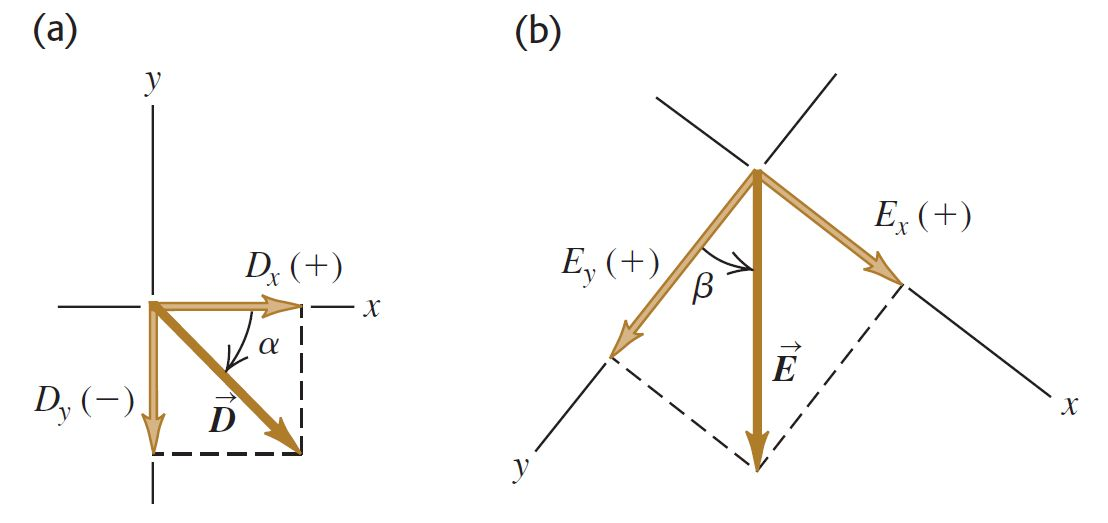
\includegraphics[height=1.7in]{images/EXAMPLE_vec_comp.jpg}
\end{center}



 \end{frame}


%%%%%%%%%%%%%%%%%%%%%%%%%%%%%%%%%%%%%%%%%%%%%%%%%%%%%%%%%%%%%%%%%%%

\begin{frame}


Adding more than one vector:

\vspace{5mm}

\begin{equation*}
\vec{R}=\vec{A}+\vec{B}+\vec{C}
\end{equation*}

\begin{equation*}
\rightarrow R_x=A_x+B_x+C_y
\end{equation*}\

\begin{equation*}
\rightarrow R_y=A_y+B_y+C_y
\end{equation*}

\begin{equation*}
\rightarrow R_y=A_z+B_z+C_z
\end{equation*}

 \end{frame}

 
%%%%%%%%%%%%%%%%%%%%%%%%%%%%%%%%%%%%%%%%%%%%%%%%%%%%%%%%%%%%%%%%%%%

\begin{frame}


Magnitude of a vector with 3 components:
\vspace{5mm}

\begin{equation*}
\lvert \vec{A} \rvert=\sqrt{A^2_x+A^2_y+A^2_z}
\end{equation*}



 \end{frame}


%%%%%%%%%%%%%%%%%%%%%%%%%%%%%%%%%%%%%%%%%%%%%%%%%%%%%%%%%%%%%%%%%%%

\begin{frame}


Test your understanding:
\vspace{3 mm}

Two vectors $\vec{A}$ and  $\vec{B}$ both lie in the xy-plane.
\vspace{3 mm}

\begin{itemize}
\item Is it possible for $\vec{A}$ to have the same magnitude as $\vec{B}$ but different
components?
\item Is it possible for $\vec{A}$  to have the same components as $\vec{B}$  but a different
magnitude?
\end{itemize}

 \end{frame}

%%%%%%%%%%%%%%%%%%%%%%%%%%%%%%%%%%%%%%%%%%%%%%%%%%%%%%%%%%%%%%%%%%%
\subsection{Unit Vectors}


%%%%%%%%%%%%%%%%%%%%%%%%%%%%%%%%%%%%%%%%%%%%%%%%%%%%%%%%%%%%%%%%%%%
\begin{frame}

\begin{itemize}
\item A unit vector is a vector that has a magnitude of 1  with no units
\pause
\item  Its only purpose is  to describe a direction in space
\pause
\item We represent them using a "hat"
\pause
\item the unit vectors that point into the direction of the coordinate axes are:
\pause




\end{itemize}



   \begin{columns}[c]
   \column{2in}  % slides are 3in high by 5in wide

\begin{equation*}
\hat{\imath},~\hat{\jmath},~and~\hat{k}
\end{equation*}

  
   \column{2in}




  \begin{center}
  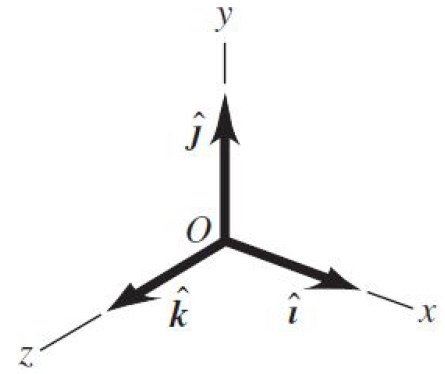
\includegraphics[height=1.3in]{images/unit_vec_1.jpg}
\end{center}


   \end{columns}





 \end{frame}

%%%%%%%%%%%%%%%%%%%%%%%%%%%%%%%%%%%%%%%%%%%%%%%%%%%%%%%%%%%%%%%%%%%
\begin{frame}

We can represent component vectors like this:
\vspace{3mm}

\begin{equation*}
\rightarrow \vec{A}_x=A_x\hat{\imath}
\end{equation*}

\begin{equation*}
\rightarrow \vec{A}_y=A_y\hat{\jmath}
\end{equation*}


\begin{equation*}
\rightarrow \vec{A}_z=A_z\hat{k}
\end{equation*}

 \end{frame}

%%%%%%%%%%%%%%%%%%%%%%%%%%%%%%%%%%%%%%%%%%%%%%%%%%%%%%%%%%%%%%%%%%%
\begin{frame}




   \begin{columns}[c]
   \column{2in}  % slides are 3in high by 5in wide

We can represent a vector using this notation:
\vspace{3mm}

\begin{equation*}
\vec{A}=\vec{A}_x+\vec{A}_y
\end{equation*}



\begin{equation*}
\rightarrow \vec{A}=A_x\hat{\imath}+A_y\hat{\jmath}
\end{equation*}



  
   \column{2in}




  \begin{center}
  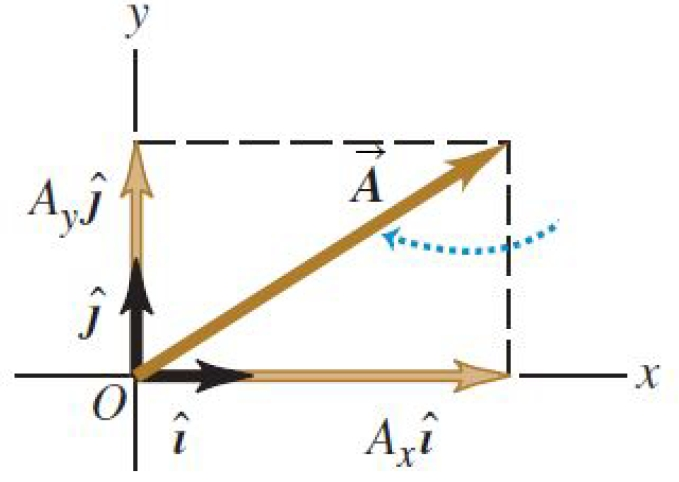
\includegraphics[height=1.6in]{images/unit_vec_2.jpg}
\end{center}


   \end{columns}



 \end{frame}

%%%%%%%%%%%%%%%%%%%%%%%%%%%%%%%%%%%%%%%%%%%%%%%%%%%%%%%%%%%%%%%%%%%
\begin{frame}

How can we represent the sum of two vectors using this notation?

\vspace{3mm}

Guess! 


 \end{frame}


%%%%%%%%%%%%%%%%%%%%%%%%%%%%%%%%%%%%%%%%%%%%%%%%%%%%%%%%%%%%%%%%%%%
\begin{frame}

Test your understanding


\vspace{3mm}


Arrange the following vectors
in order of their magnitude, with the vector of largest magnitude first.
\vspace{3mm}

\begin{enumerate}
\item $\vec{A}=(3\hat{\imath}+5\hat{\jmath}-2\hat{k})$
\item $\vec{A}=(-3\hat{\imath}+5\hat{\jmath}-2\hat{k})$
\item $\vec{A}=(3\hat{\imath}-5\hat{\jmath}-2\hat{k})$
\item $\vec{A}=(3\hat{\imath}+5\hat{\jmath}+2\hat{k})$
\end{enumerate}

 


 \end{frame}

%%%%%%%%%%%%%%%%%%%%%%%%%%%%%%%%%%%%%%%%%%%%%%%%%%%%%%%%%%%%%%%%%%%

\subsection{Review:  Functions}
%%%%%%%%%%%%%%%%%%%%%%%%%%%%%%%%%%%%%%%%%%%%%%%%%%%%%%%%%%%%%%%%%%%
\begin{frame}


   \textbf{Functions}
   \pause
   \vspace{3mm}


\begin{itemize}
\item A function is a binary relation between two sets that associates every element of the first set to exactly one element of the second set
\pause
\item some useful functions:
	\begin{enumerate}
	\item linear functions
	\item quadratic functions
	\item sin, cos
	\item exponential, logarithmic function
	\end{enumerate}

\end{itemize}


 \end{frame}
%%%%%%%%%%%%%%%%%%%%%%%%%%%%%%%%%%%%%%%%%%%%%%%%%%%%%%%%%%%%%%%%%%%
\begin{frame}


  Examples \dots
   \pause
   \vspace{3mm}

   \begin{center}
      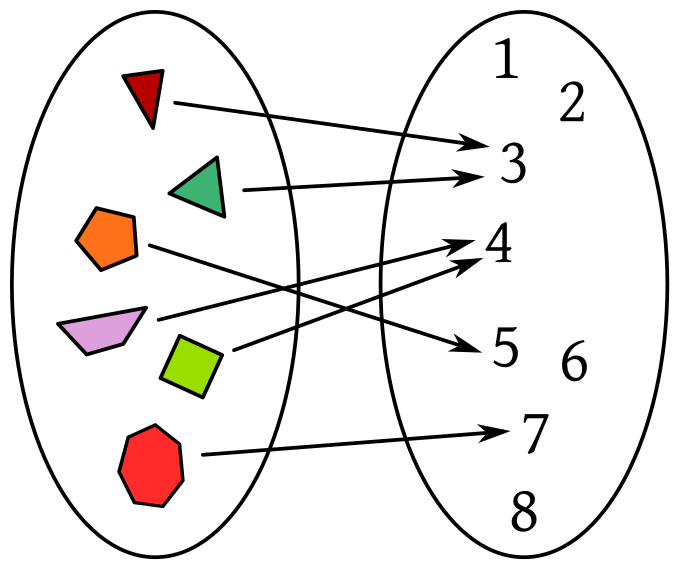
\includegraphics[height=1.5in]{images/PolygonsFunction.png}
    \end{center}


 \end{frame}

 %%%%%%%%%%%%%%%%%%%%%%%%%%%%%%%%%%%%%%%%%%%%%%%%%%%%%%%%%%%%%%%%%%%
\begin{frame}



   \vspace{3mm}
 
    \begin{center}
       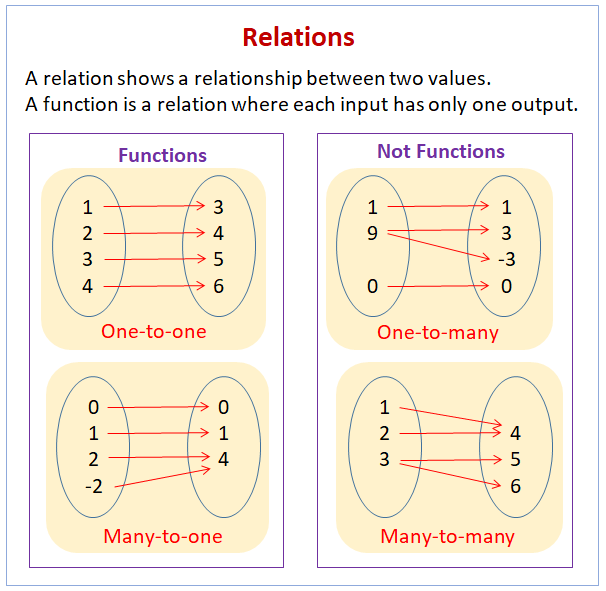
\includegraphics[height=3.in]{images/relation-function.png}
     \end{center}
 
 
  \end{frame}
 

%%%%%%%%%%%%%%%%%%%%%%%%%%%%%%%%%%%%%%%%%%%%%%%%%%%%%%%%%%%%%%%%%%%

 
 \begin{frame}


Instead of using diagrams, we can use a law to draw the function in the x-y axes \dots
\pause

\begin{equation*}
  \boxed{ y=f(x)}
\end{equation*}
 
  \end{frame}
 

%%%%%%%%%%%%%%%%%%%%%%%%%%%%%%%%%%%%%%%%%%%%%%%%%%%%%%%%%%%%%%%%%%%


\begin{frame}

Linear Functions:

\begin{equation*}
f(x)=Ax+C
\end{equation*}


\pause

   \begin{columns}[c]
   \column{2in}  % slides are 3in high by 5in wide
Representation in the xy axes coordinates:

\begin{equation*}
y=Ax+C
\end{equation*}

  
   \column{2in}




  \begin{center}
  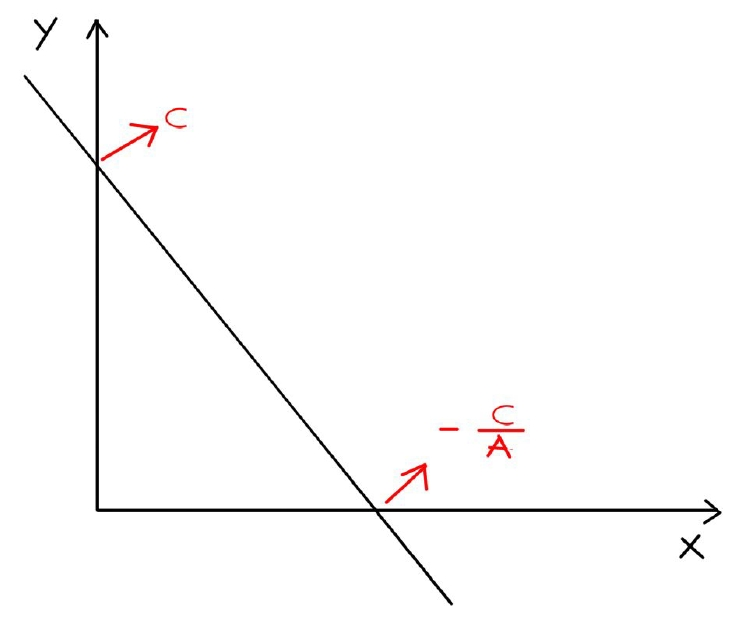
\includegraphics[height=1.5in]{images/function.jpg}
\end{center}


   \end{columns}


 \end{frame}
%%%%%%%%%%%%%%%%%%%%%%%%%%%%%%%%%%%%%%%%%%%%%%%%%%%%%%%%%%%%%%%%%%%
\begin{frame}

Cuadratic Functions:

\begin{equation*}
f(x)=ax^2+bx+c
\end{equation*}


\pause

   \begin{columns}[c]
   \column{2in}  % slides are 3in high by 5in wide
Representation in the xy axes coordinates:

\begin{equation*}
y=ax^2+bx+c
\end{equation*}

  
   \column{2in}




  \begin{center}
  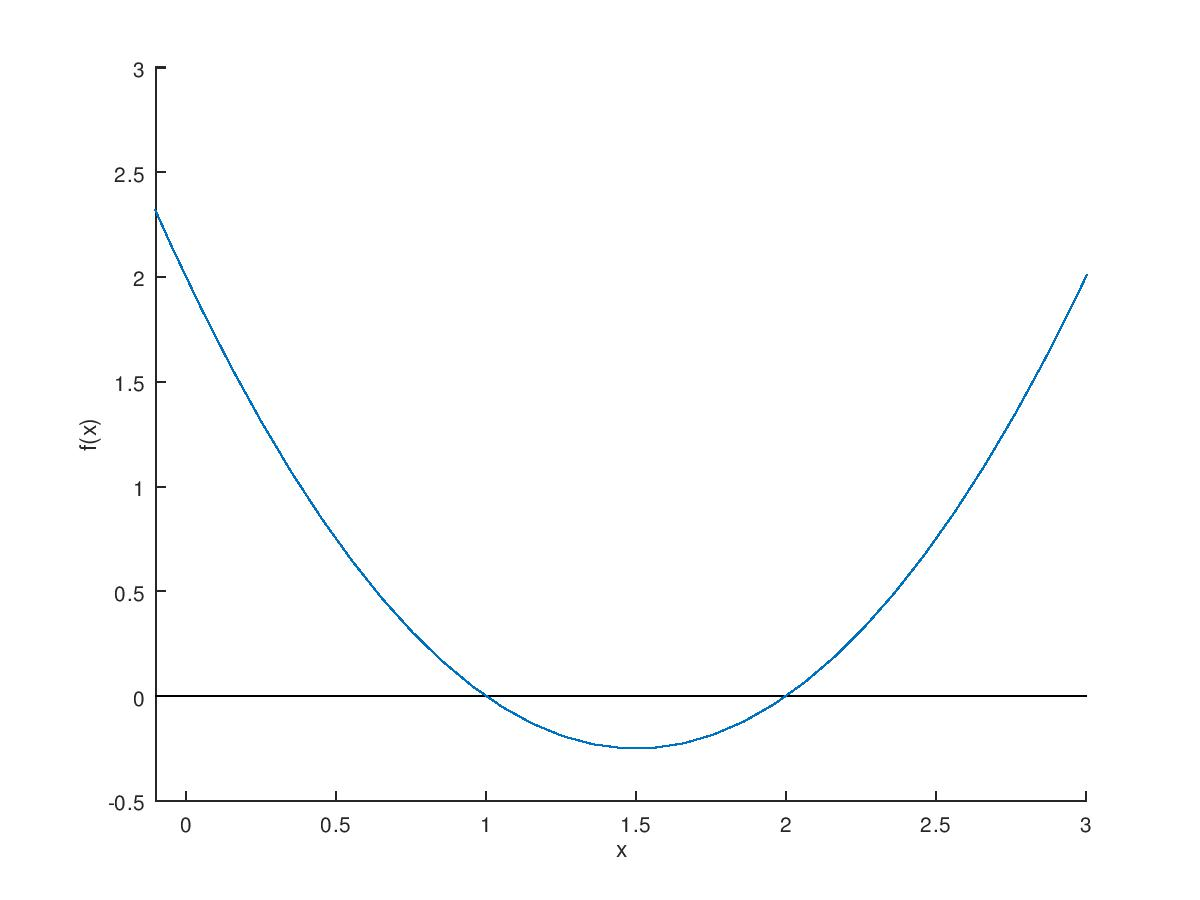
\includegraphics[height=1.5in]{images/cuadratic.jpg}
\end{center}


   \end{columns}


 \end{frame}


 %%%%%%%%%%%%%%%%%%%%%%%%%%%%%%%%%%%%%%%%%%%%%%%%%%%%%%%%%%%%%%%%%%%
\begin{frame}

   \begin{columns}[c]
      \column{2in}  % slides are 3in high by 5in wide
      Trygonometric Functions:
   

   
   \begin{equation*}
   sin(\alpha) =\frac{opposite}{hypotenuse}
   \end{equation*}
   

   
     
      \column{2.5in}
   
   
   
   
     \begin{center}
     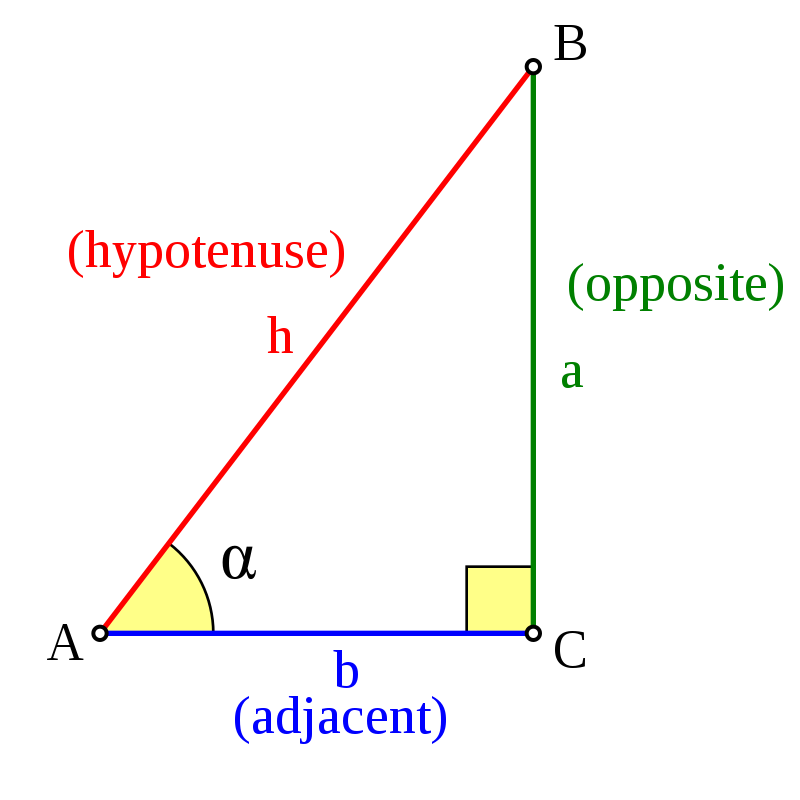
\includegraphics[height=2.3in]{images/triangle.png}
   \end{center}
   
   
      \end{columns}

 \end{frame}
 %%%%%%%%%%%%%%%%%%%%%%%%%%%%%%%%%%%%%%%%%%%%%%%%%%%%%%%%%%%%%%%%%%%
 \begin{frame}

   \begin{columns}[c]
      \column{2in}  % slides are 3in high by 5in wide
      Trygonometric Functions:
   

   
   \begin{equation*}
   cos(\alpha) =\frac{adjacent}{hypotenuse}
   \end{equation*}
   

   
     
      \column{2.5in}
   
   
   
   
     \begin{center}
     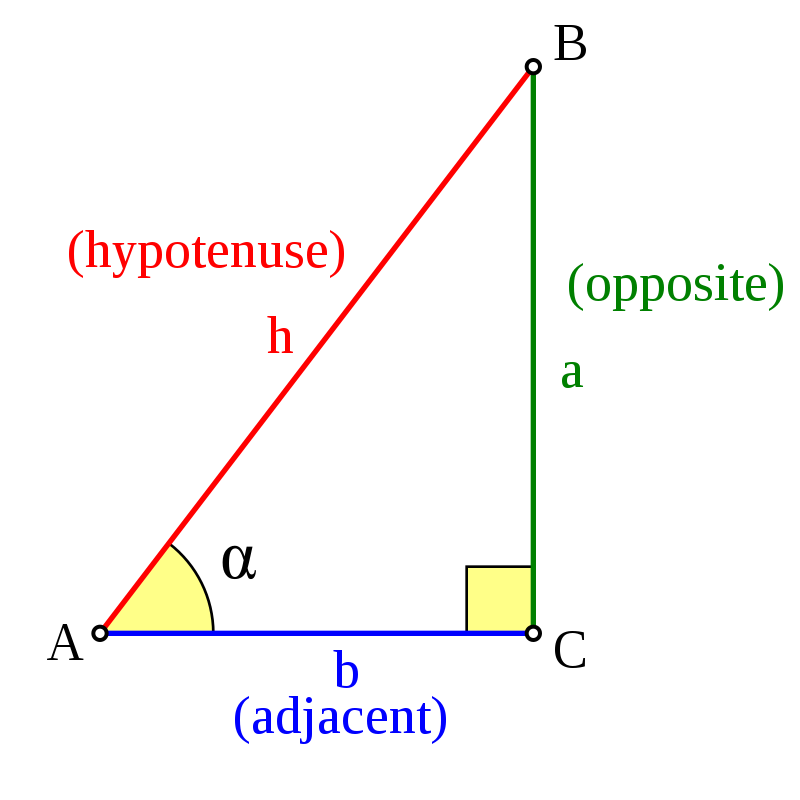
\includegraphics[height=2.3in]{images/triangle.png}
   \end{center}
   
   
      \end{columns}

 \end{frame}

  %%%%%%%%%%%%%%%%%%%%%%%%%%%%%%%%%%%%%%%%%%%%%%%%%%%%%%%%%%%%%%%%%%%
  \begin{frame}

   \begin{columns}[c]
      \column{2in}  % slides are 3in high by 5in wide
      Trygonometric Functions:
   

   
   \begin{equation*}
   tan(\alpha) =\frac{opposite}{adjacent}
   \end{equation*}
   

   
     
      \column{2.5in}
   
   
   
   
     \begin{center}
     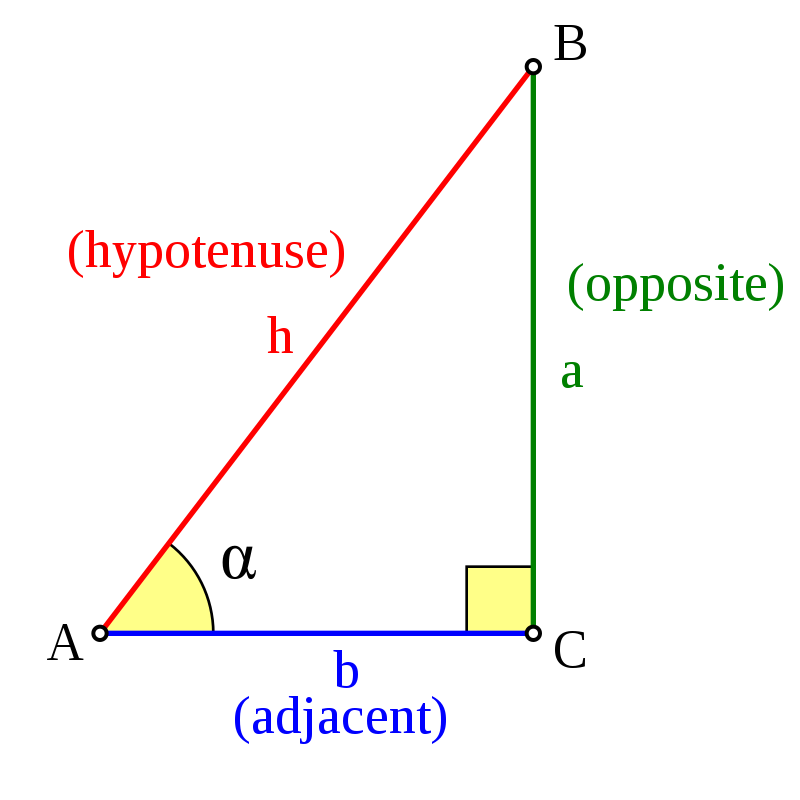
\includegraphics[height=2.3in]{images/triangle.png}
   \end{center}
   
   
      \end{columns}

 \end{frame}



%%%%%%%%%%%%%%%%%%%%%%%%%%%%%%%%%%%%%%%%%%%%%%%%%%%%%%%%%%%%%%%%%%%
\begin{frame}



   Trygonometric Functions:

   \begin{center}
      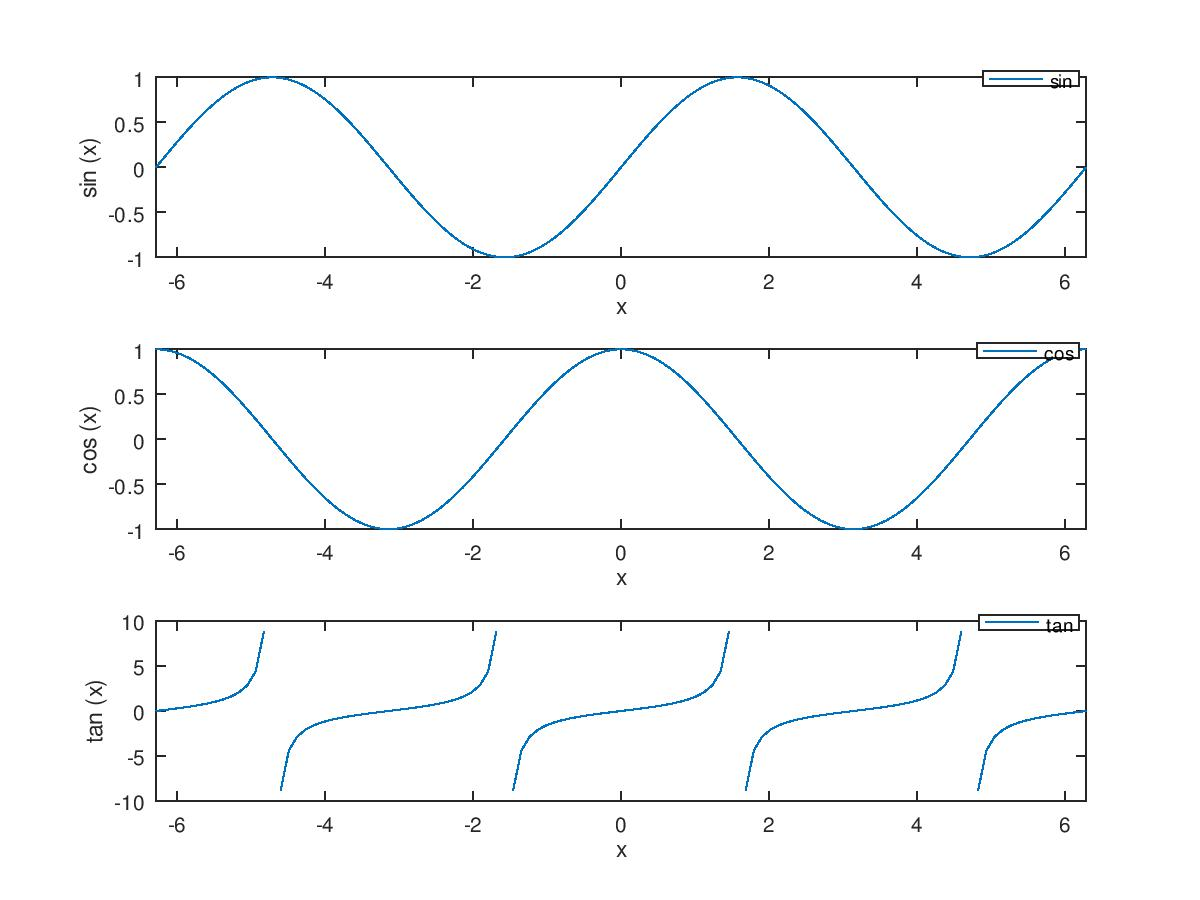
\includegraphics[height=3.in]{images/trigonometric.jpg}
    \end{center}
    

 \end{frame}


  %%%%%%%%%%%%%%%%%%%%%%%%%%%%%%%%%%%%%%%%%%%%%%%%%%%%%%%%%%%%%%%%%%%
  \begin{frame}

\textbf{Measuring angles: radians}
\vspace{3mm}

\begin{center}
   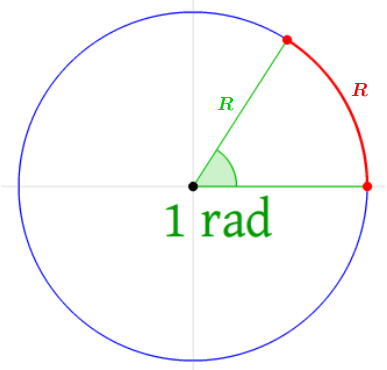
\includegraphics[height=2.in]{images/radians.png}
 \end{center}

 \end{frame}

  %%%%%%%%%%%%%%%%%%%%%%%%%%%%%%%%%%%%%%%%%%%%%%%%%%%%%%%%%%%%%%%%%%%
  \begin{frame}

   \textbf{Radians to degrees}
   \vspace{3mm}


   How many rads are 360 deg?

   \pause
   \vspace{3mm}


\begin{equation*}
   radians=\frac{arc~length}{radious}\pause =\frac{2\pi}{1}
\end{equation*}



\pause

\begin{equation*}
   2\pi~rad\rightarrow 360 deg
\end{equation*}

\begin{equation*}
   x~rad \rightarrow \frac{360}{2\pi} x\pause = \frac{180}{\pi} x
\end{equation*}


\end{frame}
   


  %%%%%%%%%%%%%%%%%%%%%%%%%%%%%%%%%%%%%%%%%%%%%%%%%%%%%%%%%%%%%%%%%%%
  \begin{frame}

   \textbf{How do I calculate the angle if I know the sin/cos/tan?}
   \vspace{3mm}

\begin{equation*}
   sin(30)=0.5\pause \rightarrow asin(0.5)= 30
\end{equation*}
\pause

\begin{equation*}
   cos(30)=0.86602540378\pause \rightarrow acos(0.86602540378)= 30
\end{equation*}

\pause

\begin{equation*}
   tan(30)=0.57735026919\pause \rightarrow atan(0.57735026919)= 30
\end{equation*}
\pause

You have to check what are the units of the angles\dots
\end{frame}
   





































%%%%%%%%%%%%%%%%%%%%%%%%%%%%%%%%%%%%%%%%%%%%%%%%%%%%%%%%%%%%%%%
 \end{document}
%%%%%%%%%%%%%%%%%%%%%%%%%%%%%%%%%%%%%%%%%%%%%%%%%%%%%%%%%%%%%%%